%
% Works for all workflows.
% If gonative is specified, dvips->ps2pdf works as well.
%
\documentclass[11pt]{article}
\usepackage{amsmath} % use only for the align environment
\usepackage[blinkonjmp,blinkonrestore,!preview,!viewMagWin]{fitr}
\usepackage{graphicx}

% Uncomment to use custom hooks, there are minimal functions already defined.
% Uncomment to see these simple examples.
%\usepackage[js=jmpHook,js=restoreHook]{lmacs}

\hypersetup
{%
    pdftitle={Jumping to a Rectangular Region},
    pdfauthor={D. P. Story},
    pdfsubject={Demo file to test the FitR view destination of PDF},
    pdfkeywords={LaTeX, PDF, Acrobat, JavaScript},
    pdfpagemode=UseNone
}

\parindent0pt \parskip6pt \pagestyle{empty}

\def\cs#1{\texttt{\char`\\#1}}

% \renewcommand{\overlayPresets}{\H{I}\S{D}\BG{}\BC{blue}}
% \renewcommand{\allowFXDefault}{false}

\begin{document}

\begin{center}\sffamily\bfseries\Large
    Jumping to a Rectangular Region\\[1ex]\normalsize\normalcolor
    Dr. D. P. Story, \href{http://www.acrotex.net}{Acro\negthinspace\TeX.NeT}
\end{center}

\textbf{Introduction.} This document demonstrates a technique designed to
help people with low vision read material by providing them with a
convenient way to magnify specific regions of the document. This is
especially useful for reading technical material such as mathematics, as
is demonstrated here.

\textbf{Instructions:} Click on any of the mathematics to magnify a region
around it, the border will blink briefly to focus your attention on it.
To restore the previous view, click on the region again,
the formula is briefly highlighted by a blinking border so
can quickly find your place in the document.


\textbf{Sample Mathematical Text.} Consider the problem of numerically
solving the first order differential equation
\jdRect*[adddestw=60,adddesth=20]{$y'=f(t,y)$} on
\jdRect*[adddestw=1in,adddesth=30]{$[t_{start}, t_{end}]$}. Suppose we
want to classify third order \textsf{Runge-Kutta} type methods. Start with
\begin{align*}
\jdRect[height=1.3in,width=2.6in,lift=16pt,shift=-15pt,adddestw=10,adddesth=10] %
K_1 &= hf(t_n, y_n)\\
K_2 &= hf(t_n +r h, y_n+aK_1)\\
K_3 &= hf(t_n +s h, y_n+bK_1+cK_2)\\
K &= w_1 K_1+ w_2 K_2+ w_3 K_3\\
y_{n+1} &= y_n+K
\end{align*}
Find the system of equations satisfied by
\jdRect*[adddestw=10,adddesth=10]{$r,s, a, b, c, w_1, w_2, w_3$}
that will make the above algorithm a third order method.

\textbf{Inline links.} Links can be provided within the text to jump to a
magnified region that needs to be inspected more closely. The links below
are different from the ones above. After jumping to a magnified rectangle,
restore the preview view by clicking on the rectangle.

\def\RungePic{\includegraphics[width=\marginparwidth]{graphics/runge}}
\def\KuttaPic{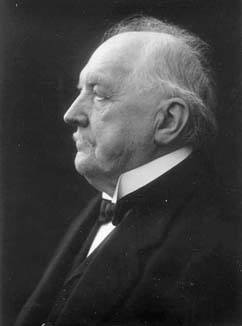
\includegraphics[width=\marginparwidth]{graphics/Kutta}}
\def\jrOpts#1#2{link=#1,dest=#2}

\textbf{\jdRect*[nodest,\jrOpts{jmp}{rungePic},adddestw=10,adddesth=10]{Carl Runge}}%
\marginpar{\jdRect*[\jrOpts{restore}{rungePic},adddestw=\marginparsep,
adddesth=\marginparpush]{\parbox[b]{\marginparwidth}{\RungePic\\
\normalcolor\centering\footnotesize\textsf{Carl Runge}}}} (1867-1944)
was the third of four sons from a well-to-do German merchant family.  He
is remembered for his \textsf{Runge-Kutta} method for solving
differential equations.

\textbf{\jdRect*[nodest,\jrOpts{jmp}{KuttaPic}]{Martin Kutta}}%
\marginpar{\jdRect*[\jrOpts{restore}{KuttaPic},adddestw=\marginparsep,
adddesth=\marginparpush]{\parbox[b]{\marginparwidth}{\KuttaPic\\
\normalcolor\centering\footnotesize\textsf{Martin Kutta}}}} (1867-1944)
extended the Runge's method of solving ordinary differential equations. He
is also known for his work on airfoils.

% Again, don't forget to press
%\textbf{Alt+Left Arrow} to return to the view you had before you clicked
%on the link.

\begin{flushright}
This work was  motivated by Mohsen M.
\end{flushright}

\newpage

\noindent\textbf{FX and verbatim text.} The \cs{jsRect*} can ``scoop up'' verbatim text. We illustrate
with several examples from the documentation.

Using the \cs{verb} command: \jdRect*[adddestw=10bp,adddesth=10bp]{\verb!#$$%&$%^&$%^$!}

% measure the width of the widest line in the verbatim listing below
\newsavebox\fitrBox
\begin{lrbox}{\fitrBox}
\verb~\renewcommand{\overlayPresets}{\H{I}\BG{}\BC{blue}\S{D}}%~%
\end{lrbox}\edef\wdDisplay{\the\wd\fitrBox}

\renewcommand{\overlayPresets}{\H{I}\BG{}\BC{blue}\S{D}}%

Jump to the \jdRect*[adddestw=10bp,adddesth=10bp]{\textsf{fitr} Package!} Click
on the verbatim region below to view the listing up close.
\restoreOverlayPresets
\begin{flushleft}
\jdRect*[adddestw=10bp,adddesth=10bp]
{\begin{minipage}{\wdDisplay}
\begin{verbatim}
\renewcommand{\overlayPresets}{\H{I}\BG{}\BC{blue}\S{D}}%
...
Jump to the \jdRect*[adddestw=10bp,adddesth=10bp]%
  {{\fitrpkg} Package!}
\end{verbatim}
\end{minipage}}
\end{flushleft}
\jdRect[width=\wdDisplay,height=4\baselineskip,lift=-\baselineskip,adddestw=10bp,adddesth=10bp]%
Now using \cs{jdRect}.\parskip0pt
%\previewOn\viewMagWinOn
\begin{verbatim}
\renewcommand{\overlayPresets}{\H{I}\BG{}\BC{blue}\S{D}}%
...
Jump to the \jdRect*[adddestw=10bp,adddesth=10bp]%
  {{\fitrpkg} Package!}
\end{verbatim}



\end{document}
